Godiva is an un-shielded, pulsed, nuclear burst reactor. It is essentially a homogeneous sphere of highly enriched uranium with a diameter of $30$ cm, that was operated by inserting a piston of fissile material~\cite{Godiva1961}. In this tutorial the critical benchmark configuration described in Ref.~\cite{GodivaBenchmark} is considered. The geometry that is modeled by THOR is a homogeneous sphere of radius $8.71$ cm discretized by tetrahedra similar to Fig.~\ref{fig:godiva_coarse} (with the exception that Fig.~\ref{fig:godiva_coarse} shows on-eighth of the domain). The energy domain is discretized with six energy groups, and cross sections are provided by~\cite{GodivaBenchmark}.

\begin{figure}[th]
  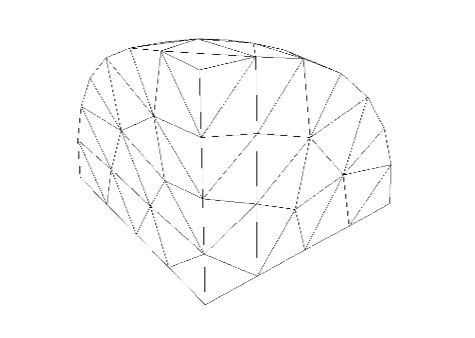
\includegraphics[width=1.0\textwidth]{chapters/godivatutorial/figures/godiva_coarse.png}
  \caption{Coarse mesh for Godiva problem, picture courtesy~\cite{FerrerPhD}}
  \label{fig:godiva_coarse}
\end{figure}

This tutorial first explains how a tetrahedral mesh is created for the Godiva problem, then the cross sections data input is discussed, and finally the standard input to THOR is covered.
The input files discussed below for the Godiva tutorial are located in:
\begin{verbatim}
    >> /home/<usr>/projects/THOR/THOR/examples/Godiva_tutorial
\end{verbatim}

\subsection{Godiva Mesh}
The workflow described here is suitable if the user has access to the Cubit mesh generator. A Cubit journal file is provided in directory:
\begin{verbatim}
    >> /home/<usr>/projects/THOR/THOR/examples/Godiva_tutorial
\end{verbatim}
It creates the exodus file \verb"godiva.e". To verify whether Cubit is available to the user on the target computer execute the command line:
\begin{verbatim}
    >> which cubit
\end{verbatim}
Note that even if Cubit is installed on the target computer it might not be available to the user unless its path is defined in the user's search paths. To execute the journal file, the last line must be modified by replacing \verb"<path>" with:
\begin{verbatim}
    /home/<usr>/projects/THOR/THOR/examples/Godiva_tutorial ..
    /create_mesh/from_cubit
\end{verbatim}
then execute Cubit with the command line:
\begin{verbatim}
    >> cubit <godiva_mesh_CUBIT.jou
\end{verbatim}
For users that do not have access to Cubit, the \verb"godiva.e" file is provided in the \verb"from_cubit" directory.
The exodus file \verb"godiva.e" is converted to THOR's native mesh format by executing the THOR mesh generator using the standard input file \verb"convert_godiva.in" that is included in the \verb"from_cubit" directory with the command line:
\begin{verbatim}
    >> /home/<usr>/projects/THOR/pre-processors/THOR_Mesh_Generator/Thor_Mesh_Generator_MP.exe -i convert_godiva.in
\end{verbatim}
In this case this input file contains the following lines:
\begin{verbatim}
./godiva_1_o.e
./godiva_1_o.thrm
\end{verbatim}
specifying the input exodus file and the THOR mesh formatted output file. The mesh conversion infers the file format of the input by the filename extension; currently \verb".e" and \verb".gmsh" for exodus and gmesh formats, respectively, are supported. The conversion is performed by typing:
\begin{verbatim}
    /home/<usr>/projects/THOR/pre-processors/THOR_Mesh_Generator/ ...
    Thor_Mesh_Generator.exe -i convert_godiva.in
\end{verbatim}
After successful completion of the conversion, the following printout should appear:
\begin{verbatim}
============================================================

   TTTTTTT  HH     HH  OOOOO  RRRRRR
     TTT    HH     HH OOOOOOO RRRRRRR
     TTT    HH     HH OO   OO RR   RR
     TTT    HHHHHHHHH OO   OO RRRRRR
     TTT    HHHHHHHHH OO   OO RRRR
     TTT    HH     HH OO   OO RR RR
     TTT    HH     HH 0000000 RR  RR
     TTT    HH     HH  OOOOO  RR   RR

   Tetrahedral High Order Radiation Transport Code

   By North Carolina State University

   Version 1.0 - Update 2020
============================================================

============================================================
Executing -->THOR_MESH_GENERATOR<-- application
============================================================

------------------------------------ Input ------------------------------------
Infile mesh file name: ./godiva_1_o.msh
Output mesh file name: ./godiva_1_o.thrm
Mesh refinement level:    0

No region ID edits are provided
No source ID edits are provided
No boundary ID edits are provided


============================================================
Application -->THOR_MESH_GENERATOR<-- terminated successfully
============================================================
\end{verbatim}

The file \verb"godiva_1_o.thrm" should result from this execution for use by THOR. This concludes the mesh generation step for this tutorial.

\subsection{Cross section data}
The THOR cross section file for the Godiva benchmark is provided by:
\begin{verbatim}
    /home/<usr>/projects/THOR/THOR/examples/Godiva_tutorial/cross_sections/godiva.xs
\end{verbatim}
THOR uses a custom cross section format that is explained in detail in Sec.~\ref{sec:THOR_format}.

\subsection{THOR input file and executing THOR}
The THOR input file is
\begin{verbatim}
   /home/<usr>/projects/THOR/THOR/examples/Godiva_tutorial/...
   THOR/godiva.i
\end{verbatim}
THOR uses a keyword-based input that is listed in Sect.~\ref{sec:THOR_format}. The Godiva tutorial input file is now explained in detail; note that this listing includes comments separated by \verb"#" at the end of each line that are not present in the original input file.
\begin{verbatim}
Godiva 6 group example              # title line

  start problem                     # beginning of problem block
    execution = yes                 # problem is solved
    lambda = 0                      # constant approximation (SC)
    type = keig                     # solve an eigenvalue problem
    keigsolver = pi ; piacc = none  # Power iterations w/o
                                    # acceleration, note separation
                                    # by ; to have same-line synatx
    sweep = precomp                 # sweep path precomputed
    page_refl = save                # reflected bnd fluxes stored
    kconv = 1E-8                    # stopping tolerance on k-eff
    innerconv = 1E-12              # stopping tolerance inner it
    outerconv = 1E-7                # stopping tolerance outer it
    maxinner = 4 ; maxouter = 5000  # max # inner/outer it
  end problem                       # terminate the problem block

  start inout                       # start input/output file block
    mesh_file =  ../create_mesh/from_CUBIT/godiva_1_o.thrm  # mesh file
    xs_file =  ../cross_sections/godiva.xs  # XS file
    flux_file = godiva.flux         # plain flux output file
    vtk = flux mat                  # print flux and mat ids to vtk
    print_xs = yes                  # XS are echoed
  end inout.                        # terminate this block

  start cross_sections
     ngroups = 6                    # the number of energy groups
     upscattering = no              # upscattering is not present
                                    # scat. XS is lower triangular
  end cross_sections

  start quadrature
    qdtype = levelsym               # level-symmetric quadrature
    qdorder = 4                     # order 4
  end quadrature

  start regionmap                   # the region map maps block
     1                              # ids to materials; in this
                                    # case the only block is
  end regionmap                     # assigned material 1 that is
                                    # present in XS file

end file                            # the input file is terminated
                                    # by "end file"
\end{verbatim}

The Godiva tutorial is solved with THOR via the command line:
\begin{verbatim}
    >> /home/<usr>/projects/THOR/THOR/thor-1.0.exe -i godiva.i
\end{verbatim}

Completion of execution of the Godiva tutorial is indicated by the printout:
\begin{verbatim}
--------------------------------------------------------
    Execution of THOR completed successfully
 --------------------------------------------------------
\end{verbatim}

THOR provides the following output that is discussed in this tutorial:
\begin{itemize}
    \item The final estimate of the multiplication factor is printed under ``Execution Summary'', ``Final eigenvalue''. In this case the value is $0.9611$. This is not close to critical because the mesh that
    is created does not conserve the volume of the critical sphere. When creating a tetrahedral mesh,
    Cubit places the nodes on the sphere's surface, but that necessarily leads to the volume of the discretized geometry to be smaller than the original volume. In this case, the computational volume
    is $2742.4\text{ cm}^3$, while the actual volume is $2767.8\text{ cm}^3$.
    \item A summary of group-wise, region-averaged reaction rates is provided for each region identifier separately under ``Region averaged reaction rates''. The volume of each region, and group-wise fluxes, fission, absorption, and fission source rates are listed.
    \item Two vtk formatted files, \verb"flux.vtk" contains spatial flux maps, and \verb"mat.vtk" contains the material map. These files can be opened with the paraview post-processing tool that is available \href{https://www.paraview.org/download/}{here}.
\end{itemize}

The reaction rate summary is given by:
\begin{verbatim}
--------------------------------------------------------
    Region averaged reaction rates
--------------------------------------------------------

-- Region --   1 Volume=   2.742401E+03

   Group          Flux       Fission    Absorption      Fiss Src
       1  8.424948E-01  1.399140E-01  4.946487E-02  1.399140E-01
       2  1.573081E+00  2.333728E-01  9.509448E-02  2.333728E-01
       3  9.814645E-01  1.379655E-01  5.968679E-02  1.379655E-01
       4  1.631588E+00  2.215631E-01  1.006868E-01  2.215631E-01
       5  1.198341E+00  1.915944E-01  9.089592E-02  1.915944E-01
       6  1.792724E-01  4.652155E-02  2.413688E-02  4.652155E-02
Total     6.406241E+00  9.709313E-01  4.199657E-01  9.709313E-01
\end{verbatim}

The results can be improved greatly by enforcing volume conservation on the Cubit mesh. This is accomplished manually in this tutorial by changing the radius in the Cubit journal file to .